% !Mode:: "TeX:UTF-8"

%%%中文版式与英文版式通过参数设置
\documentclass{ctacn}%英文版式

%可以选择使用times字体
\usepackage{newtxtext}
\usepackage{hhline}
\usepackage{ctex}
\begin{document}


%%%%%%%输入年、月、卷、期
\Volume{xxxx}{x}{xxx}{xx}{x}
\cndoi{1001-0920(0000)00-0000-00}
\doi{10.13195/j.kzyjc.0000.0000}
\paperdate{xxxx-xx-xx}{xxxx-xx-xx}%接收日期,修回日期
%%%%%%%设置开始页
\setcounter{page}{1}

%%%%%%%输入页眉显示的题目

%%%%%%%%%%
%%%                  本刊为匿名审稿,新投稿时不要填写任何作者信息,包括所有位置的姓名、单位以及邮箱
%%%%%%%%%%%%
\runheading{基于DropOut降噪自编码的磨矿系统故障诊断}%页眉设置,填写第一作者及论文题目
\xiangmujijin{国家自然基金项目(00000000)}%项目基金  为空会自动取消显示

\authorintro{曲星宇\,(1984$-$), 男,博士研究生,高级工程师,所长.研究领域为大型工业设备自动控制、网络控制系统.;曾鹏 (1976$-$),男,博士,研究员,博士生导师,室主任.研究领域为无线传感器网络、工业无线通信.}%作者简介,填写第一作者和导师的简介         %新投稿不修改
\authorcor{E-mail: quxingyu\_qxy@163.com}%通讯作者邮箱,新投稿不修改


%%%-------------中文信息---------------
\cntitle{基于DropOut降噪自编码的磨矿系统故障诊断} %输入中文标题


%                  新投稿不要修改下面的姓名及单位
%%%中文作者和单位,\dag代表通信作者,“作者一”代表3个字的名,“作者”代表2个字的名
\cnauthor{曲星宇\makebox{$^{1,2,3\dag}$} , ~~曾~~~~鹏\makebox{$^{1,2}$} ,~~徐承成\makebox{$^{4}$} ,~~付东东\makebox{$^{4}$}}%新投稿不修改
{(1.中国科学院沈阳自动化研究所工业信息学重点实验室,沈阳~110016;2.中国科学院大学,北京~100049;\\3.北方重工集团有限公司,沈阳~110178;4.东北大学 信息科学与工程学院,沈阳~110004)}%%省会城市无需加省%%新投稿不要修改

%%%中文摘要
\cnabstract{目前磨矿系统的故障诊断主要依靠工人的经验,而这为故障诊断增加了大量不确定性。此外,磨矿系统的数据较为复杂,不仅工人难以对故障的发生进行准确判断,传统机器学习算法也由于数据的线性不可分而表现不佳。为了解决线性不可分的问题,我们使用神经网络进行故障分类;面对故障数据的高复杂度,为提高神经网络的表达能力,我们使用自动编码器增加网络深度;为减弱深层网络带来的过拟合现象,引入DropOut 降噪自编码,最终DropOut降噪自编码网络对于故障的分类准确率达到90.4\%。}

%%%中文关键词
\cnkeyword{故障诊断;自动编码器;DropOut;降噪自编码;Softmax分类器;深度学习}

%%%分类号、标识码
\clc{TP273}%中文分类号
\wenxianbiaoshi{A}%文献标志码

%%%%%%%----------------英文信息------------
\entitle{DropOut Denoising Autoencoder-based Fault Diagnosis for Grinding System}


%%%%%%%              新投稿不要修改下面的英文名及单位
\enauthor{QU Xing-yu\makebox{$^{1,2,3\dag}$} , ~~ZENG Peng\makebox{$^{1,2}$} ,~~XU Cheng-cheng\makebox{$^{4}$} ,~~FU Dong-dong\makebox{$^{4}$}}{
(1. Key Laboratory of Industrial Informatics, Shenyang Institute of Automation, Chinese Academy of Sciences 110016, China;2.University of Chinese Academy of Sciences, Beijing 100049, China;3.Northern Heavy Industries Group Co. Itd, Shenyang 110860, China 4.College of Information Science and Engineering,Northeastern University,Shenyang 110004,China.)}


\enabstract{The current fault diagnosis of the grinding system relies mainly on the experience of the workers, which adds a lot of uncertainty to the fault diagnosis. In addition, the grinding system data is too complex, which makes it hard for the workers to judge, and brings about poor performance for traditional machine learning algorithms due to the linear indivisiblity. In order to solve the problem of linear indivisibility, we use neural network for fault classification. In the face of the high complexity of fault data, we use autoencoder to increase network depth in order to improve the expression ability of neural network. To reduce the over-fitting brought about by deep network, we introduce DropOut and denoising autoencoder. Ultimately, the Dropout Denoising Autoencoder (DDA) reached the accuracy of 90.4\% to the fault classification.}

\enkeyword{Fault Diagnosis;Autoencoder;DropOut;Denoising Autoencoder;Softmax Classifier;Deep Learning}

\maketitle




\begin{multicols}{2}
\section{引\quad 言}
磨矿过程是选矿厂生产过程的最重要环节之一,其主要任务是将矿石经过物理的研磨和分级,使有用矿物与脉石单体解离,为后续的选别作业创造条件。

磨矿过程是典型的流程工业过程,生产过程缓慢,滞后时间长,其机理复杂、影响因素多,如给矿量、给水量、原矿性质及装球量等随机变化及各种外界干扰因素,往往造成磨矿过程工作不稳定。现有磨矿分级过程核心设备球磨机的运行监控还仅仅停留在对数据的显示和存储上,没有完整的故障诊断系统为设备的稳定运行保驾护航,根本原因也在于人员因素和技术因素,矿山环境大多恶劣偏僻,难以吸引专业技术人员,而故障诊断的基础是通过操作人员的经验积累人工判断来实现的,而人为控制的过程由于受到种种外界条件的干扰,会对控制结果产生直接或间接的影响。

本文基于以上问题,使用DropOut降噪自编码算法,实现对V型磨矿系统工作过程中故障智能诊断。本文首先对采集点长期以来采集到的数据集,对其进行数据预处理,接下来,搭建传统BP神经网络、设置网络参数,输入为没有进行任何特征变换的特征向量,训练网络最终输出的结果效果并不理想,发现对于高维输入特征向量传统BP神经网络收敛速度慢且辨识效果差。

为了解决传统BP神经网络对高维输入特征向量辨识能力差的问题,在特征向量输入网络之前用自动编码器先进行特征的进一步提取,并将提取到的特征进行非线性变换。在自动编码器网络后面分别级联传统BP网络或Softmax分类器,对构建好的新网络进行训练来对故障进行预测,通过实验进行对比,可以得出结论:在故障预测准确率方面AutoencoderSoftmax(A-S)和AutoencoderBP(A-BP)深度学习网络要优于BP神经网络。然而,原始的自动编码器有着抗干扰性能较弱,泛化能力不强,并且有一定过拟合的缺陷,最后我们分别加入DropOut和使用降噪自编码,并将二者结合到一起,进行对比,最终明显提升了分类准确率。

本文中神经元网络和自编码网络层数及神经元数量为经过多次试验得到,方法为先使用3层网络,逐个增加隐藏层单元节点数量,通过3-fold方法交叉检验进行调优。当准确率不再上升的时候以当前网络结构为基础增加网络层数,继续试验,直到准确率不再上升为止。使用这种方法可以获得使网络分类最有效的最小网络结构。

\section{相关工作}
随着工业生产指标的不断提高,故障诊断技术也得到了一定程度的发展,从实现方法角度来看,故障诊断方法可以分成两大类:基于数学模型的故障诊断方法、基于人工智能的故障诊断方法。其中,基于数学模型的故障诊断方法有:

文献\textsuperscript{[1]}提出具有复杂数据特性的工业过程的多元统计监视方法,并分别讨论了基于数据和基于知识方法进行故障诊断的优势、进展、适用范围及二者结合的可能。

文献\textsuperscript{[2]} 提出利用未知输入观测器与著名的Beard故障检测滤波器结合的有效故障诊断方法,主要是通过观测器估计系统输出,然后将它与输出的测量值作比较从中获得故障信息。

基于数学模型的故障诊断方法对于系统的数学模型线性度有很大的依赖性,导致其有很大的局限性,而近些年出现的基于人工智能的故障诊断方法可以很好的弥补这一缺点。基于神经网络的人工智能型诊断方法,将某一问题的若干知识表示在同一网络中,通用性高、便于实现并行联想推理。

文献\textsuperscript{[3]}采用多层感知器神经网络和系统辨识相结合的方法,运用Matlab系统辨识工具箱和神经网络工具箱,提出了由线性模型和非线性补偿模型组成的混合模型结构的精矿品位预报方法,建立了精矿品位预报模型。

传统的神经网络模型,优点为分类的准确度高,有较强的鲁棒性和容错能力,能够处理复杂的非线性函数并充分逼近复杂的非线性关系,并且能发现不同输入间的依赖关系;缺点为需要大量的参数,学习过程无法观察且学习时间长。

文献\textsuperscript{[4]}基于自动编码器容易受噪声干扰而拟合噪声信息,导致过拟合的特点,通过在训练过程中随机将节点的连接权变为0的方式引入噪声,提出了降噪自编码,显著地提高了分类器的性能,以无监督的方式在一些情况下超越了深度信念网络。

文献\textsuperscript{[5, 6]}引入了DropOut技术,通过在训练过程中随机丢弃节点,使用了来自不同“稀疏”网络的进行训练。在测试时,通过简单地使用具有较小权重的单个无连网的网络来估计所有这些稀疏网络的预测的平均效果。这显着减少过度拟合并对其他正则化方法有着重大改进。最终该方法在图像识别、语音分类等领域都实现了最先进的效果。

文献\textsuperscript{[7]}提出了基于深度网络的电力变压器故障诊断方法,工程实例测试结果表明,该方法正确可行,诊断性能优于三比值、神经网络和支持向量机的方法,适用于电力变压器的故障诊断。

综上所述方法各有优缺点和其各自的适用性。深度学习可以较好地拟合数据,而缺点为对数据量的需求过大,数据量不足会导致严重的过拟合。这正适用于由于球磨机数据的特点:大数据、多变量、强耦合和大惯性。本文采用Autoencoder和Softmax结合的深度学习算法,并加入降噪与DropOut来实现对大数据分析研究并预测故障类型。使用自动编码器对数据进行压缩,可以解决高维数据的处理压力。通过实验证明,引入降噪与DropOut可以显著降低过拟合、提高网络泛化能力。

\section{基于BP网络进行故障检测}

\subsection{数据与处理及分析}
本文依托V型磨矿系统岗位记录提供的数据集,通过对数据集的分析实现对磨矿系中所现的故障进行预测。数据集的形式为每隔一个小时系统在采集点(温度、压力、声音、振动等)所采集到的数据,共计1024个小时,30种测量指标。

在数据预处理的过程中,首先剔除无效(即数值并不改变的)数据,数据集由30维下降为24维。对于数据集中的缺失数据,本文填入缺失数据点前后5小时的数据的均值。

磨矿生产过程中的故障一般分为磨矿设备如球磨机的故障和生产工艺故障如物料输入输出的失衡等。本文主要针对项目所给数据集中的故障进行分析,最终的目的是要对故障进行诊断,因此,这些故障的类型被看作标签(label)。对于这些数据的表征,本文采用“one-hot”编码,标签编码如表1。


\begin{center}
	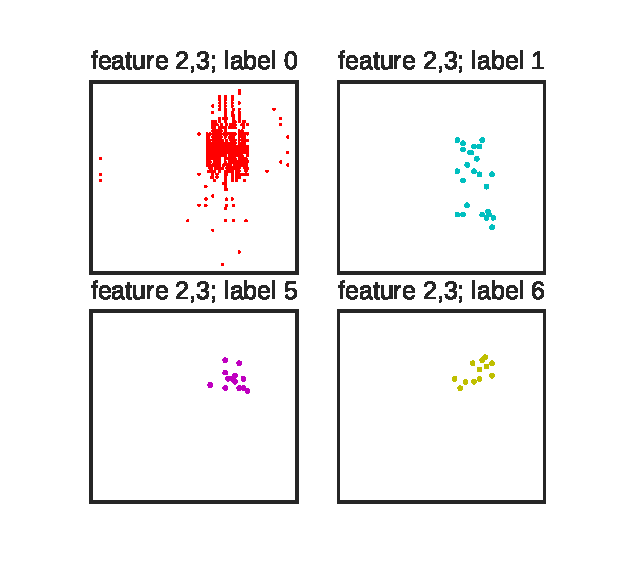
\includegraphics[scale=0.7, trim=0 0 0 0]{figs/data_features}\\
	\label{fig1}
	\figcaption{第0.1维特征分类图}
\end{center}

由表1可以看出,故障共7类,加上无故障共8种,其中的几类有较强的相关性,不易辨识。通过分析数据发现:1024组数据中有877类为无故障,147类为有故障,为严重的分类不均衡,因此,分类器的正确率不宜作为评判指标。这里我们选择了其中的两维特征分析如图1所示。


\subsection{BP网络的建立}

人工神经网络对数据的拟合能力较强,因此我们将神经网络技术应用于磨矿生产过程中的诊断,从而获得理想的诊断效果。目前应用较多前馈型网络的是BP网络,其学习速度快,容易训练,逼近能力和分类能力强。本文使用BP神经网络来对磨矿中的故障进行诊断,诊断系统功能结构如图2所示。

\begin{center}
	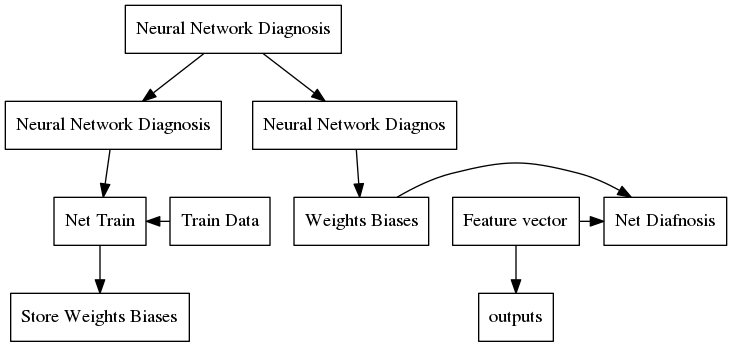
\includegraphics[scale=0.12, trim=0 0 0 0]{figs/procedure}
	\label{fig2}
	\figcaption{磨矿神经网络故障诊断功能示意图}
\end{center}
\end{multicols}
\begin{center}
	\tabcaption{故障原因及表征方法表}
	\renewcommand\tabcolsep{12.6pt}%调整表格长度
	\label{tab1}
	\renewcommand\tabcolsep{10pt}
	\begin{tabular}{ccc}\toprule
	故障现象&故障原因&故障表征\\
	\hline
	正常&无&10000000\\
	给矿压力低&进料端矿箱漏矿&01000000\\
	给矿压力增大&旋流器穿孔&00100000\\
	主电机电流低,离合器气罐压力低&气缸故障&00010000\\
	主电机前后轴瓦、邮箱温度高,高压供油压力低&稀油站冷却水阀门损坏&00001000\\
	主轴瓦给料右温度上升,供油压力给料右下降&油压低,轴瓦温度高&00000100\\
	主轴瓦排料右温度升高,供油流量排料下降低&流量低,轴瓦温度升高&00000010\\
	主电机温度高&油温高,油压低&00000001\\
	\bottomrule
	\end{tabular}
\end{center}
\begin{multicols}{2}

\subsection{实验与结果分析}

本文分别采用$1024\times24$维的整体数据集划分为$900\times24$维的数据作为训练样本集,剩下的$124\times24$维数据作为测试集,进行验证可以防止网络过拟合。在训练样本集输入到网络时,进行分批处理,即每次输入$32\times24$维的数据,训练好网络后保存其权重和阈值,测试集再输入到训练好的网络中,来验证网络可靠性和诊断的准确率。

\begin{center}
	\tabcaption{混淆矩阵表}
	\label{tab:2}
	\begin{tabular} {cccc}\toprule
		\multirow{2}{*}[-2pt]{}&\multirow{2}{*}[-2pt]{}&\multicolumn{2}{c}{预测结果}\\
		\cmidrule(lr){3-4}
		&&$+1$&$-1$\\\hline
		\multirow{2}{*}[-2pt]{真实结果}&$+1$&真正例(TP)&伪反例(FN)\\
		&$-1$&伪正例(FP)&真反例(TN)\\
		\bottomrule
\end{tabular}\end{center}

训练样本集输入后网络的输出从大的层面上讲分为两类:一是有无故障;二是已经判断出来有故障,对于有故障的数据接下来进行进一步的分析是哪一类故障。本文中的故障辨识问题不是传统的分类问题,其存在着严重的分类不均衡问题。在非均衡分类中的主要评价指标可以利用混淆矩阵给出,如表2所示。


本文中将有故障当作正例,没有故障当作反例,使用了如下评价指标:

(1)错误率$S_1$:
\begin{align}
S_1=1-\frac{TP+TN}{TP+FP+TN+FN}
\end{align}


(2)预测有故障正确率$S_2$(正例正确率):
\begin{align}
S_2=\frac{TP}{TP+FP}
\end{align}

(3)预测无故障正确率$S_3$(反例正确率):
\begin{align}
S_3=\frac{TN}{TN+FN}
\end{align}

由于本问题的分类非常不均衡,错误率仅为一个参考评价指标。对传统的BP神经网络进行实验验证。本文采用的神经元网络激活函数为Sigmoid函数,节点规模为$24\rightarrow100\rightarrow8$实验结果如下:


\begin{center}
	\tabcaption{BP神经网络实验结果}
	\label{tab:3}
	\begin{tabular} {cccc}\toprule
		\multirow{2}{*}[-2pt]{}&\multirow{2}{*}[-2pt]{}&\multicolumn{2}{c}{预测结果}\\
		\cmidrule(lr){3-4}
		&&有故障&无故障\\\hline
		\multirow{2}{*}[-2pt]{真实结果}&有故障&21&24\\
		&无故障&24&55\\
		\bottomrule
\end{tabular}\end{center}

在本例中,预测有故障的正确率为46.7\%,无故障的正确率为69.6\%,错误率为38.7\%。可以看出,如果对于输入的特征向量不作任何特征变化就输入到神经网络中,网络在有无故障的辨识正确率方面表现都比较差。这也进一步说明传统BP神经网络不适用高维输入的非均衡分类问题。

\section{原始自动编码器}

本文中的24维训练样本对于神经网络来说唯独过高,训练困难采取特征压缩的技术对数据进行无监督地特征提取。基于此,我们使用自动编码器。自编码神经网络是一种无监督学习算法,以神经元网络的层状结构为基础,在训练时它让其输出值等于输入值,通过隐藏层进行稀疏性限制或限制隐藏层的规模达到特征压缩的效果。

本文建立的编码网络结构为$24\rightarrow150\rightarrow8\rightarrow150\rightarrow24$,各层神经元的激活函数选为RELU函数。训练完成后取出自动编码器结构为$24\rightarrow150\rightarrow8$的前一半作为编码器,输出层接一个Softmax分类器就形成了结构为$24\rightarrow150\rightarrow8\rightarrow8$的A-S分类器网络。训练算法为L-BFGS,初始学习率为0.01,目标函数为使得“交叉熵”最小。

\subsection{试验网络的建立}

在进行实验时,选择其中909组数据作为训练样本集,余下的115组数据作为测试集来进行验证。在24维特征向量输入网络之前,利用自编码网络对其进行特征提取,将特征降低为8维。

训练完自动编码器之后,在隐藏层特征之后加入Softmax分类器,得到最终分类网络结构为$24\rightarrow150\rightarrow24\rightarrow8$,利用表4中的数据带入上面的公式可以得到A-S深度学习网络预测有故障的正确率为82.2\%,预测无故障的正确率为88.5\%,而错误率降低为13.9\%。

\subsection{试验结果}

\begin{center}
	\tabcaption{A-S实验结果}
	\label{tab:5}
	\begin{tabular} {cccc}\toprule
		\multirow{2}{*}[-2pt]{}&\multirow{2}{*}[-2pt]{}&\multicolumn{2}{c}{预测结果}\\
		\cmidrule(lr){3-4}
		&&有故障&无故障\\\hline
		\multirow{2}{*}[-2pt]{真实结果}&有故障&37&8\\
		&无故障&8&62\\
		\bottomrule
\end{tabular}\end{center}

由上述结果可知,A-S深度学习网络在预测有无故障正确率方面明显优于前面两种网络,此外还大大降低了错误率,由此可以看出该深度学习网络对分均衡分类问题有着良好的分类效果。

\section{引入DropOut与降噪自编码}
从图3也能看出,传统自动编码器对数据的恢复效果一般,而且使用测试集测试自动编码器编码的时候,编码效果明显弱于训练集。这是因为自动编码器对噪声数据有着一定的过拟合。为了解决这个困难,我们引入DropOut与降噪自编码技术。为了便于对比,网络规模和结构与上一章的自动编码器一致。

\subsection{DropOut}

DropOut是一种通用的训练神经网络并能明显降低过拟合的方法。在训练过程中,将神经网络中的神经元按照一定概率$P(d)$丢弃,训练这些稀疏的模型,并去掉权值惩罚项,将其替换为限制权值的截断上限。因为噪声通常表现为高频干扰,用这种方法既可以将对高频干扰的拟合钳位,又可以以较低成本实现模型融合的效果。在测试过程中,将输入校正为为$1-P(d)$倍,使得神经网络传输的数据均值不变。

\subsection{降噪自编码}
降噪自编码通过将输入数据加入随机干扰,或将输入数据的某些维度随机置零。训练时要求即便加入了干扰,仍够可以还原输入。通过这种方法,可以使自动编码器无监督地能学习到更加鲁棒的高层特征,克服噪声的干扰,显著减少神经网络对噪声的拟合。在自动编码器训练时,随机对编码器(即输入层)的输入元素随机置0,而解码器要求能够重建原始输入(即未置0的输入)信息。通过实验证明该方法可以大幅消除噪声造成的影响,减弱过拟合。

\subsection{实验与结果分析}

在对改进自动编码器的行实验时,选择900组数据作为训练样本集,余下的124组数据作为测试集来进行验证。为方便比较,使用与之前的自动编码器相同网络结构,DropOut 概率选择0.5,在训练编码器的时候加入;降噪时随即丢弃单元时每个节点被丢弃的概率为0.1。

\subsubsection{DropOut自动编码器实验结果}

由表5可以计算出加入DropOut之后网络对于有故障预测的准确率为88.7\%,而对于无故障预测的正确率为84.8\%,错误率也下降为11.3\%。可以看出,使用DropOut 之后可以显著减少过拟合,对样本进行正确拟合之后,泛化能力得到显著改善。

\begin{center}
	\tabcaption{DropOut自动编码器实验结果}
	\label{tab:6}
	\begin{tabular} {cccc}\toprule
		\multirow{2}{*}[-2pt]{}&\multirow{2}{*}[-2pt]{}&\multicolumn{2}{c}{预测结果}\\
		\cmidrule(lr){3-4}
		&&有故障&无故障\\\hline
		\multirow{2}{*}[-2pt]{真实结果}&有故障&39&6\\
		&无故障&7&63\\
		\bottomrule
\end{tabular}\end{center}

\subsubsection{DropOut降噪自编码实验结果}

利用表6中的数据可以得到DropOut降噪自编码网络预测有故障的正确率为90.4\%,预测无故障的正确率为88.6\%,而错误率降低为9.6\%。经过降噪自编码与DropOut的共同作用,完善地解决了之前容易过拟合的困难,使准确率达到工业界先进水平。

\begin{center}
	\tabcaption{DropOut降噪自编码实验结果}
	\label{tab:8}
	\begin{tabular} {cccc}\toprule
		\multirow{2}{*}[-2pt]{}&\multirow{2}{*}[-2pt]{}&\multicolumn{2}{c}{预测结果}\\
		\cmidrule(lr){3-4}
		&&有故障&无故障\\\hline
		\multirow{2}{*}[-2pt]{真实结果}&有故障&39&6\\
		&无故障&5&65\\
		\bottomrule
\end{tabular}\end{center}

\section{结\quad 论}

本文使用DropOut降噪自编码,在A-S深度学习网络的基础上,显著降低了分类错误率,达到工业界最先进的水平。这种方法避免了传统基于神经网络的方法容易陷入过拟合的困境,对数据进行深层特征提取,实现了数据降噪,提高了分类神经网络的鲁棒性,将为今后的非传统分类问题提供一个理论依据,并将在深度学习实现故障辨识领域产生深远意义。


\begin{thebibliography}{99}
\addtolength{\itemsep}{-0.7em}
% \bibliographystyle{bib/gbt7714-2005}
% \bibliography{bib/reference.bib}
\bibitem[1]{1} 刘强, 柴天佑, 秦泗钊, 等. 基于数据和知识的工业过程监视及故障诊断综述[J]. 控制与决策, 2010 (6): 801-807.\\
(LIU Qiang, CHAI Tian-you, QIN S Joe, et al. Progress of data-driven and knowledge-driven process monitoring and fault diagnosis for industry process[J]. CONTROL AND DECISION, 2010 (6): 801-807.)

\bibitem[2]{2} Darby M L, Nikolaou M, Jones J, et al. RTO: An overview and assessment of current practice[J]. Journal of Process Control, 2011, 21(6) : 874 – 884.

\bibitem[3]{3} Garrido J, Vázquez F, Morilla F. An extended approach of inverted decoupling[J]. Journal of Process Control, 2011, 21(1) : 55 – 68.

\bibitem[4]{4} Vincent P, Larochelle H, Lajoie I, et al. Stacked denoising autoencoders: Learning useful representations in a deep network with a local denoising criterion[J]. Journal of Machine Learning Research, 2010, 11(Dec) : 3371 – 3408.

\bibitem[5]{5} Srivastava N, Hinton G E, Krizhevsky A, et al. Dropout: a simple way to prevent neural networks from overfitting.[J]. Journal of Machine Learning Research, 2014, 15(1) : 1929 – 1958.

\bibitem[6]{6} Hinton G E, Srivastava N, Krizhevsky A, et al. Improving neural networks by preventing co-adaptation of feature detectors[J]. arXiv preprint arXiv:1207.0580, 2012.

\bibitem[7]{7} 石鑫, 朱永利, 宁晓光, 等. 基于深度自编码网络的电力变压器故障诊断 [J]. 电力自动化设备, 2016, 36(5) : 122 – 126.\\
(SHI Xin, ZHU Yongli, NING Xiaoguang, et al. Transformer fault diagnosis based on deep auto-encoder network  [J]. Electric Power Automation Equipment, 2016, 36(5) : 122 – 126.)

\end{thebibliography}\vspace{-20pt}

\editor{X~~~~X}
\end{multicols}
\end{document}
